\section{Introducción \label{sec:sec1}}
El presente trabajo se basa en conocimiento de Ingeniería de Software \textit{(Software Engineering)} y el proceso denominado Descubrimiento del Conocimiento \textit{(Knowledge Discovery)}. En el presente capítulo se exponen las definiciones de ambos campos, así como también los conceptos de cada área del conocimiento en Ciencias de la Computación.

\section{Ingeniería de Software \label{sec:software_engieering}}
De acuerdo a la \textit{Association for Computer Machinery} \cite{acm}, de ahora en adelante A.C.M., Ingeniería de Software o \textit{Software Engineering}, en adelante S.E., se preocupa de la construcción y mantención de software que posee las siguientes características:

\begin{enumerate}
  \item Comportamiento confiable y eficiente.
  \item Existe el modo de poder seguir desarrollando sobre ellos y al mismo tiempo mantenerlos.
  \item Satisfacen todos los requerimientos definidos por las necesidades de los clientes.
\end{enumerate}

Por su parte, \textit{Institute of Electrical and Electronics Engineers}, de ahora en adelante I.E.E.E. \cite{ieee} define S.E. como la aplicación de un enfoque sistemático, disciplinado y cuantificable para el desarrollo, operación y mantenimiento de software, es decir, la aplicación de ingeniería al software.

\subsection{Modelos y Ciclos de Vida del Desarrollo de Software \label{sec:software_engieering_models}}

A lo largo de la historia de S.E. se ha creado una diversidad de modelos o ciclos de vida para la creación y mantención de software. Cada modelo define la forma o estrategia en que las distintas actividades del proceso deben ser llevadas a cabo para el desarrollo y mantención del producto de software. A continuación se analizan los enfoques más descritos en la literatura actual.

\subsubsection{Modelo Cascada \label{sec:cascade_model}}

Este enfoque define una secuencia lineal de pasos para la creación de un software. Las etapas suelen incluir análisis de requisitos del sistema, análisis de requisitos de software, diseño preliminar, diseño, codificación, pruebas y mantenimiento. La siguiente ilustración muestra las etapas mencionadas anteriormente.

\begin{figure}[ht]
	\begin{center}
  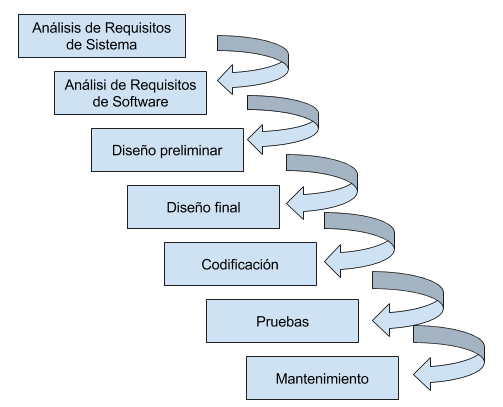
\includegraphics[width=0.5\textwidth]{./figures/chapter_02/01_cascade_phases.png}
  \setcaptioncitation{PENDIENTE}
  \caption{Fases del Modelo Cascada}
  \label{fig:cascade_model_phases}
	\end{center}
\end{figure}

El modelo de cascada se caracteriza por sus fases secuenciales, las cuales deben terminar de modo completo antes de iniciar una nueva. Adicionalmente, posee un fuerte enfoque en el levantamiento de requerimientos antes de iniciar cualquier actividad de código o de implementación del software, por lo cual se caracteriza por una intensa comunicación con los clientes o stakeholders en las fases iniciales, para luego dar protagonismo a las fases de codificación, pruebas y mantenimiento.

\textbf{Ventajas}
\begin{enumerate}
  \item Simple, permite una clara visualización de avance del proyecto.
  \item Se genera buena documentación que permite una clara planificación de los eventos dentro del proyecto.
  \item Etapa de codificación sólo se enfrenta después de tener un diseño robusto.
\end{enumerate}

\textbf{Desventajas}
\begin{enumerate}
  \item No es flexible frente a los cambios y deseos del cliente.
  \item Los errores sólo pueden ser detectados en etapas tardías de implementación.
  \item Cambios en los requerimientos agregan altísimos costos adicionales.
\end{enumerate}

\subsubsection{Modelo Incremental\label{sec:incremental_model}}

Este modelo consiste en una evolución del anterior mejorando la flexibilidad y al mismo tiempo disminuyendo  el tiempo de interacción con los stakeholders a lo largo de todo el proyecto. Con estos objetivos en mente, en vez de crear un proceso con etapas aisladas, se crea un proyecto que  puede ser diseñado, desarrollado e implementado en etapas sucesivas, incorporando al mismo tiempo la retroalimentación del cliente en etapas intermedias \cite{masssey}. El siguiente esquema ejemplifica la filosofía de este nuevo enfoque:

\begin{figure}[ht]
	\begin{center}
  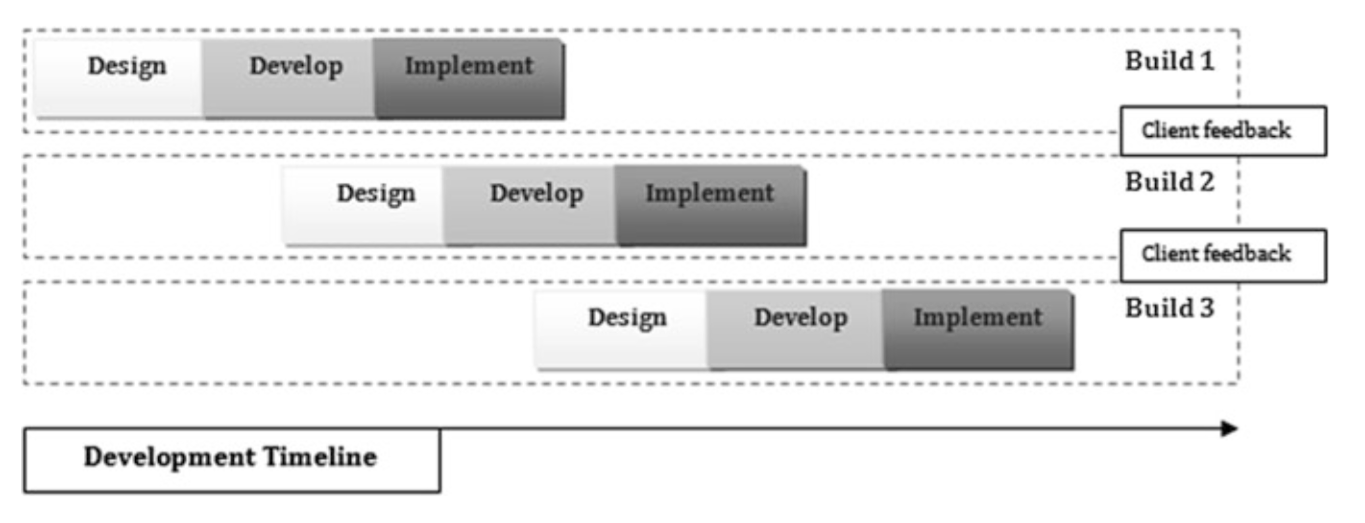
\includegraphics[width=\textwidth]{./figures/chapter_02/02_example_of_incremental_lyfe_cicle.png}
  \setcaptioncitation{PENDIENTE}
  \caption{Ejemplo de Ciclo de Vida del Modelo Incremental}
  \label{fig:cascade_incremental_model}
	\end{center}
\end{figure}

\textbf{Ventajas}
\begin{enumerate}
  \item Incorpora flexibilidad al permitir incorporar necesidades que no fueron previstas o consideradas en la etapa inicial del proyecto.
  \item Permite el desarrollo progresivo del proyecto hasta que está completo validando con los stakeholders durante todo el proyecto y no cuando éste haya finalizado.
\end{enumerate}

\textbf{Desventajas}
\begin{enumerate}
  \item La flexibilidad permitida por el proyecto puede hacer el proyecto más costoso debido a los constantes cambios que pueden realizarse.
  \item Al  incorporar nuevos elementos, debido a las etapas incrementales, puede tener problemas de incompatibilidad con versiones anteriores del software.
\end{enumerate}

\subsubsection{Rapid Application Development (RAD) \label{sec:incremental_model}}
Esta filosofía de desarrollo se basa en la idea de que los métodos desarrollados hasta los inicios de los 90 símplemente eran muy rígidos, en consecuencia no se podían aplicar de forma eficiente cuando las fechas de entrega cobran importancia. La ideología se basa en la  entrega rápida de software mientras se mantiene una alta calidad en la implementación desarrollada. Esta metodología fue desarrollada y formalizada por James Martin en el mismo horizonte de tiempo.

Este proceso de creación posee dos modalidades, la primera consiste en 4 fases secuenciales de tiempo : planificación de requerimientos, diseño desde el punto de vista del usuario, construcción y transición a la siguiente fase. En la segunda modalidad se fusionan las fases de planificación de requerimientos y diseño en una sola de análisis. Todas las fases de desarrollo en ambas modalidades se desarrolla en un espacio de tiempo determinado denominado timebox, donde se priorizan las actividades en función de las necesidades del negocio sin importar el desafío técnico al cual se ven enfrentadas \cite{gottesdiener}. A continuación se presenta un posible esquema de trabajo bajo esta metodología:

\begin{figure}[ht]
	\begin{center}
  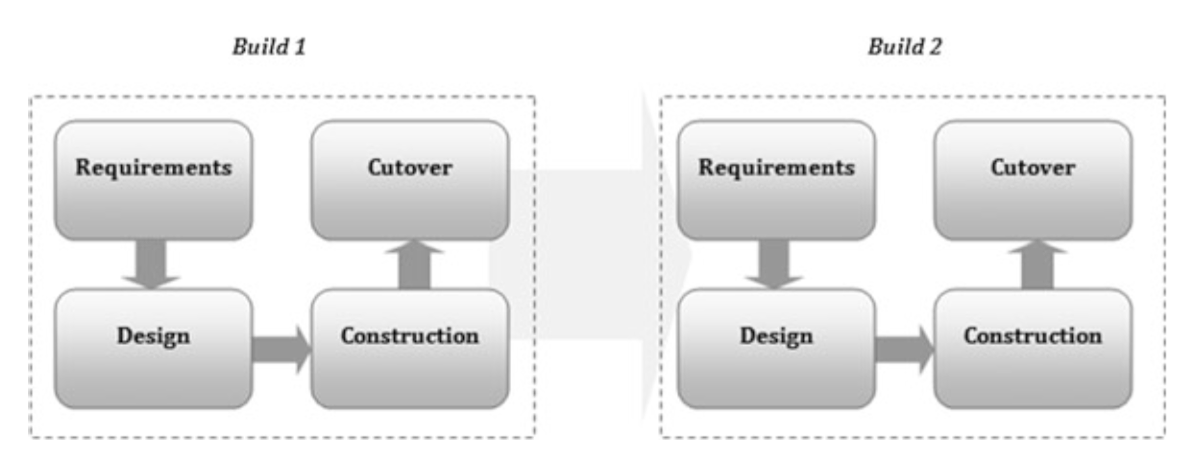
\includegraphics[width=\textwidth]{./figures/chapter_02/03_succession_of_increments.png}
  \setcaptioncitation{PENDIENTE}
  \caption{Sucesión de Incrementos en Timebox de 4 (o 3) pasos}
  \label{fig:succession_of_increments}
	\end{center}
\end{figure}

\textbf{Ventajas}
\begin{enumerate}
  \item Al enfocarse en prioridades de negocio sin importar dificultades técnicas permite entregar una implementación que satisface las necesidades más críticas de los \textit{stakeholders}.
  \item Al tener un tiempo específico de desarrollo se mantiene un paso a producción marcado por hitos.
  \item Debido a que los espacios de tiempo de desarrollo entre bloques no son necesariamente del mismo horizonte temporal es posible adaptarlos a las nuevas necesidades que vayan surgiendo en el transcurso del proyecto.
  \item Posee una comunicación constante para el desarrollo de cada fase.
\end{enumerate}

\textbf{Desventajas}
\begin{enumerate}
  \item Sólo puede ser usada cuando las personas que lo desarrollan tienen un alto nivel técnico y una gran capacidad de trabajo en equipo, debido a que los tiempos de desarrollo necesitan ser lo más preciso posible por cada bloque.
  \item Es posible que se creen expectativas falsas por parte de las personas que gestionan el proyecto al ser trabajado bajo espacios específicos de tiempo, lo que podría generar discusiones internas con el equipo de desarrollo.
\end{enumerate}

\subsubsection{Enfoque Ágil \label{sec:incremental_model}}

Esta modalidad de desarrollo nace específicamente en el año 2001 con la publicación del Manifiesto Ágil, en donde se da a conocer un \textit{framework} de cómo construir un software en un ambiente de constantes cambios y al mismo tiempo mantener un alto nivel de calidad de implementación y satisfacción al cliente. Existen 12 principios declarados en este manifiesto, los cuales pueden ser resumidos en las siguientes declaraciones \cite{agile}:

\begin{enumerate}
  \item La satisfacción del cliente es la principal prioridad.
  \item Cambios en los requerimientos son bienvenidos, no son más un obstáculo.
  \item El \textit{software} es entregado regularmente en constantes \textit{release}.
  \item Los responsables de negocio y los desarrolladores trabajamos juntos de forma cotidiana durante todo el proyecto.
  \item Individuos motivados son una pieza vital para el éxito del proyecto.
  \item Conversaciones cara a cara es esencial para una exitosa colaboración.
  \item El \textit{software} funcionando es la medida principal de progreso.
  \item El desarrollo sostenible debe ser alentado.
  \item Enfocado en bases técnicas y diseño de calidad.
  \item Simplicidad debe ser favorecida.
  \item La mejor forma de gestionar un proyecto es con equipos auto organizados.
  \item Debe haber constantes discusiones para el mejoramiento del equipo.
\end{enumerate}

En términos generales es posible establecer 4 etapas para el desarrollo bajo este enfoque  \cite{agile}:

\begin{description}
  \item[1. Selección y aprobación del proyecto] Los stakeholders (administradores, desarrolladores, clientes, entre otros) definen de modo conjunto el alcance, propósito y requerimientos del producto o implementación.
  \item[2. Iniciación del proyecto] El equipo de trabajo es construido en base a los requerimientos anteriormente establecidos. Adicionalmente, se establece la infraestructura de trabajo y se procede a la instalación de las herramientas tecnológicas a ocupar. En general, se establecen espacios de tiempo de trabajo para el equipo y reuniones de acuerdo a las necesidades del proyecto.
  \item[3. Construcción basada en iteraciones] Las iteraciones consisten en dos etapas, planificación y construcción. La idea es que al final de cada iteración se obtenga una pieza de software terminada.
  \item[4. Entrega de producto maduro \textit{(product release)}] Esta fase final está caracterizada nuevamente por dos etapas, pruebas y mejoramiento así como también de la documentación necesaria para el entendimiento del proyecto.
\end{description}

El esquema \ref{fig:agile_development_life_cycle} muestra el proceso genérico bajo cualquier proceso con enfoque ágil:

\begin{figure}[ht]
	\begin{center}
  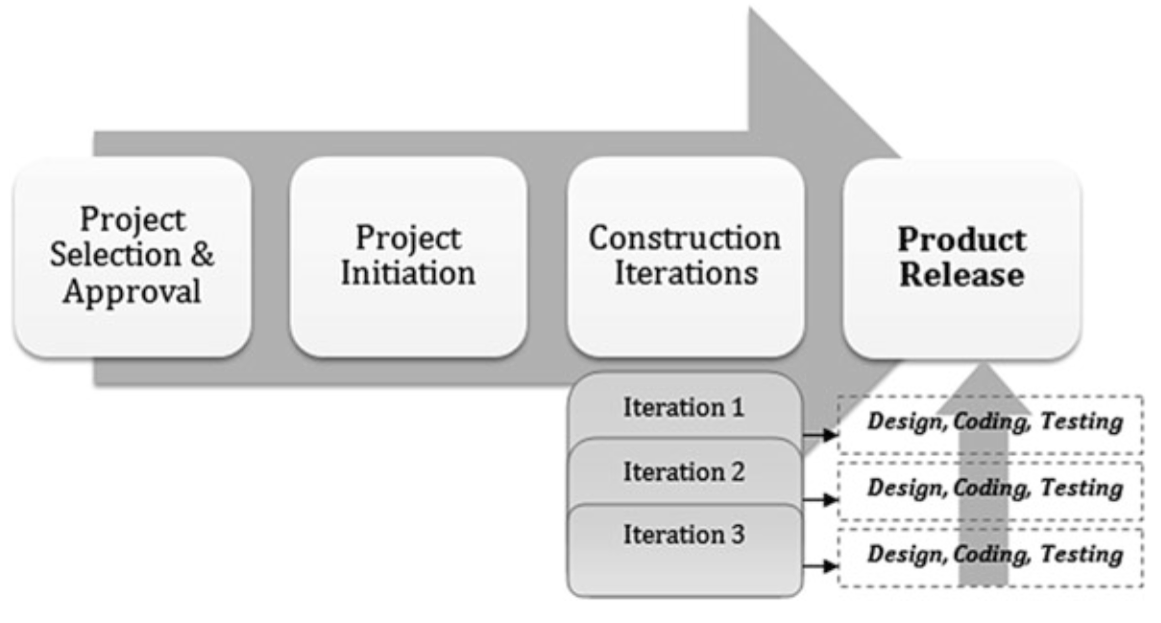
\includegraphics[width=0.85\textwidth]{./figures/chapter_02/04_agile_development_life_cycle.png}
  \setcaptioncitation{PENDIENTE}
  \caption{ Ejemplo del Ciclo de Vida del Desarrollo Ágil}
  \label{fig:agile_development_life_cycle}
	\end{center}
\end{figure}

\subsection{Metodologías de Desarrollo de Software \label{sec:methodologies}}

Un modelo o ciclo de vida puede ser considerado como una estructura de referencia, una estrategia general para enfrentar el desarrollo, pero no prescribe el modo concreto de llevarlo a cabo. La forma específica de cómo llevar a cabo el proyecto la define una metodología orientada por un determinado modelo o enfoque.

Dentro de los modelos mencionados anteriormente él más relevante hoy en día es enfoque ágil debido a los cambios que ha sufrido la industria tanto a nivel tecnológico como social. Desde su nacimiento en el año 2001 por la declaración del Manifiesto Ágil han surgidos diversas metodologías, las cuales enfrentan diferentes desafíos impuestos por los supuestos de esta modalidad de desarrollo, tales como incorporación de cambios en cualquier momento del proyecto. A continuación se describen dos de las metodologías más populares que permiten implementar el enfoque ágil, éstas son Scrum y Extreme programming (XP). La figura \ref{fig:agile_methodologies_used} muestra la dominancia de Scrum entre las metodologías ágiles:

\begin{figure}[ht]
	\begin{center}
  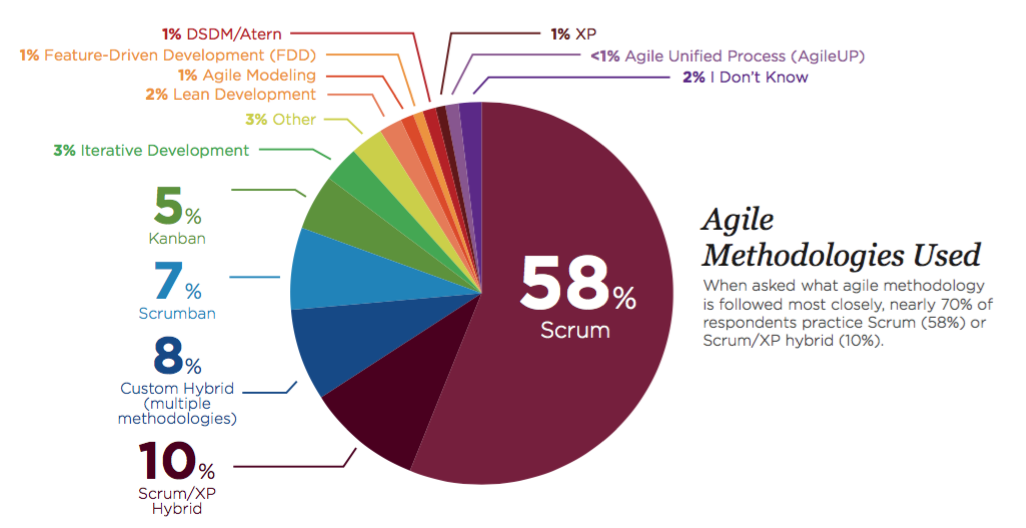
\includegraphics[width=0.85\textwidth]{./figures/chapter_02/05_agile_methodologies_used.png}
  \setcaptioncitation{PENDIENTE}
  \caption{Uso de Metodologías Ágiles}
  \label{fig:agile_methodologies_used}
	\end{center}
\end{figure}

Como se aprecia sólo Scrum cubre más del $50\%$ de la industria. Si bien XP representa sólo un $1\%$, es la base de Scrum/XP Hybrid que es usado por $10\%$ de la industria y es muy usada en grupos pequeños de desarrollo. Por lo tanto, en el desarrollo de este trabajo se consideraron tanto Scrum como XP.

\subsubsection{Scrum \label{sec:scrum}}

Esta metodología se basa principalmente en cómo un equipo debe funcionar y las relaciones que los miembros de éste establecen. Para lograr este objetivo se definen roles, eventos, artefactos y reglas. Cada componente dentro de este marco de referencia sirve para un propósito específico que son esenciales para éxito de su aplicación \cite{scrum_guide}. A continuación se ilustra la forma de trabajo en esta metodología en dos aspectos, primero la figura \ref{fig:scrum} se identificación los elementos presente en la metodología y a continuación en la figura \ref{fig:scrum_framework} se muestra cómo estos interactúan en el transcurso de un proyecto.

\begin{figure}[ht]
	\begin{center}
  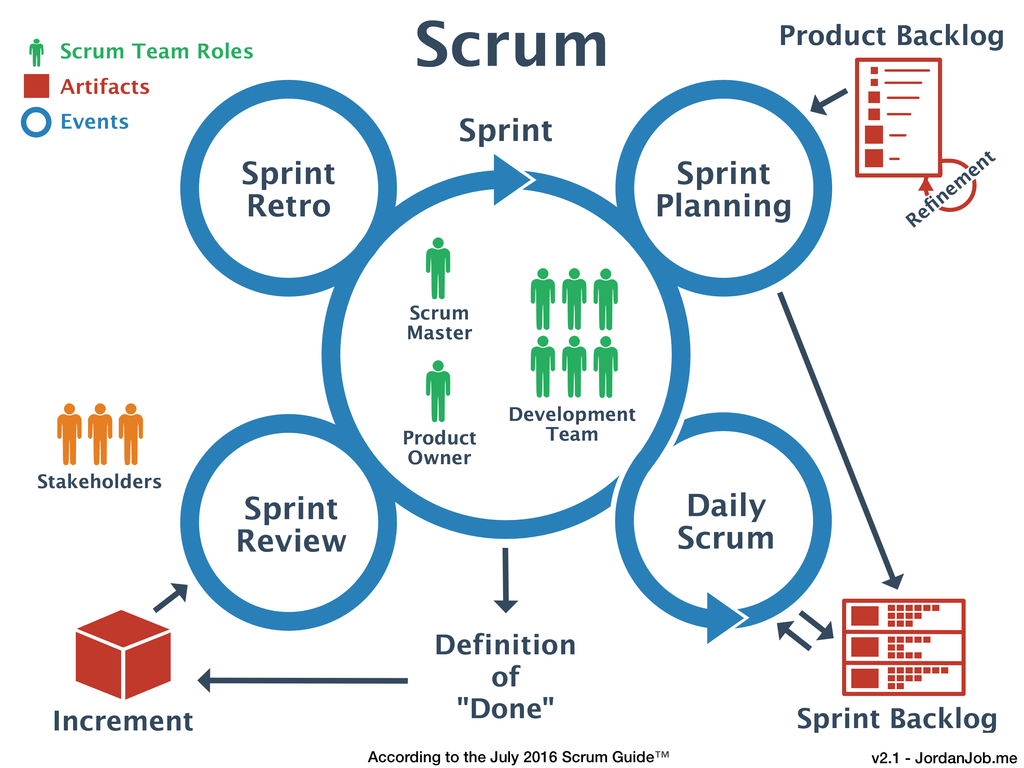
\includegraphics[width=0.85\textwidth]{./figures/chapter_02/06_scrum.png}
  \setcaptioncitation{PENDIENTE}
  \caption{Elementos presenten en Scrum}
  \label{fig:scrum}
	\end{center}
\end{figure}

\begin{figure}[ht]
	\begin{center}
  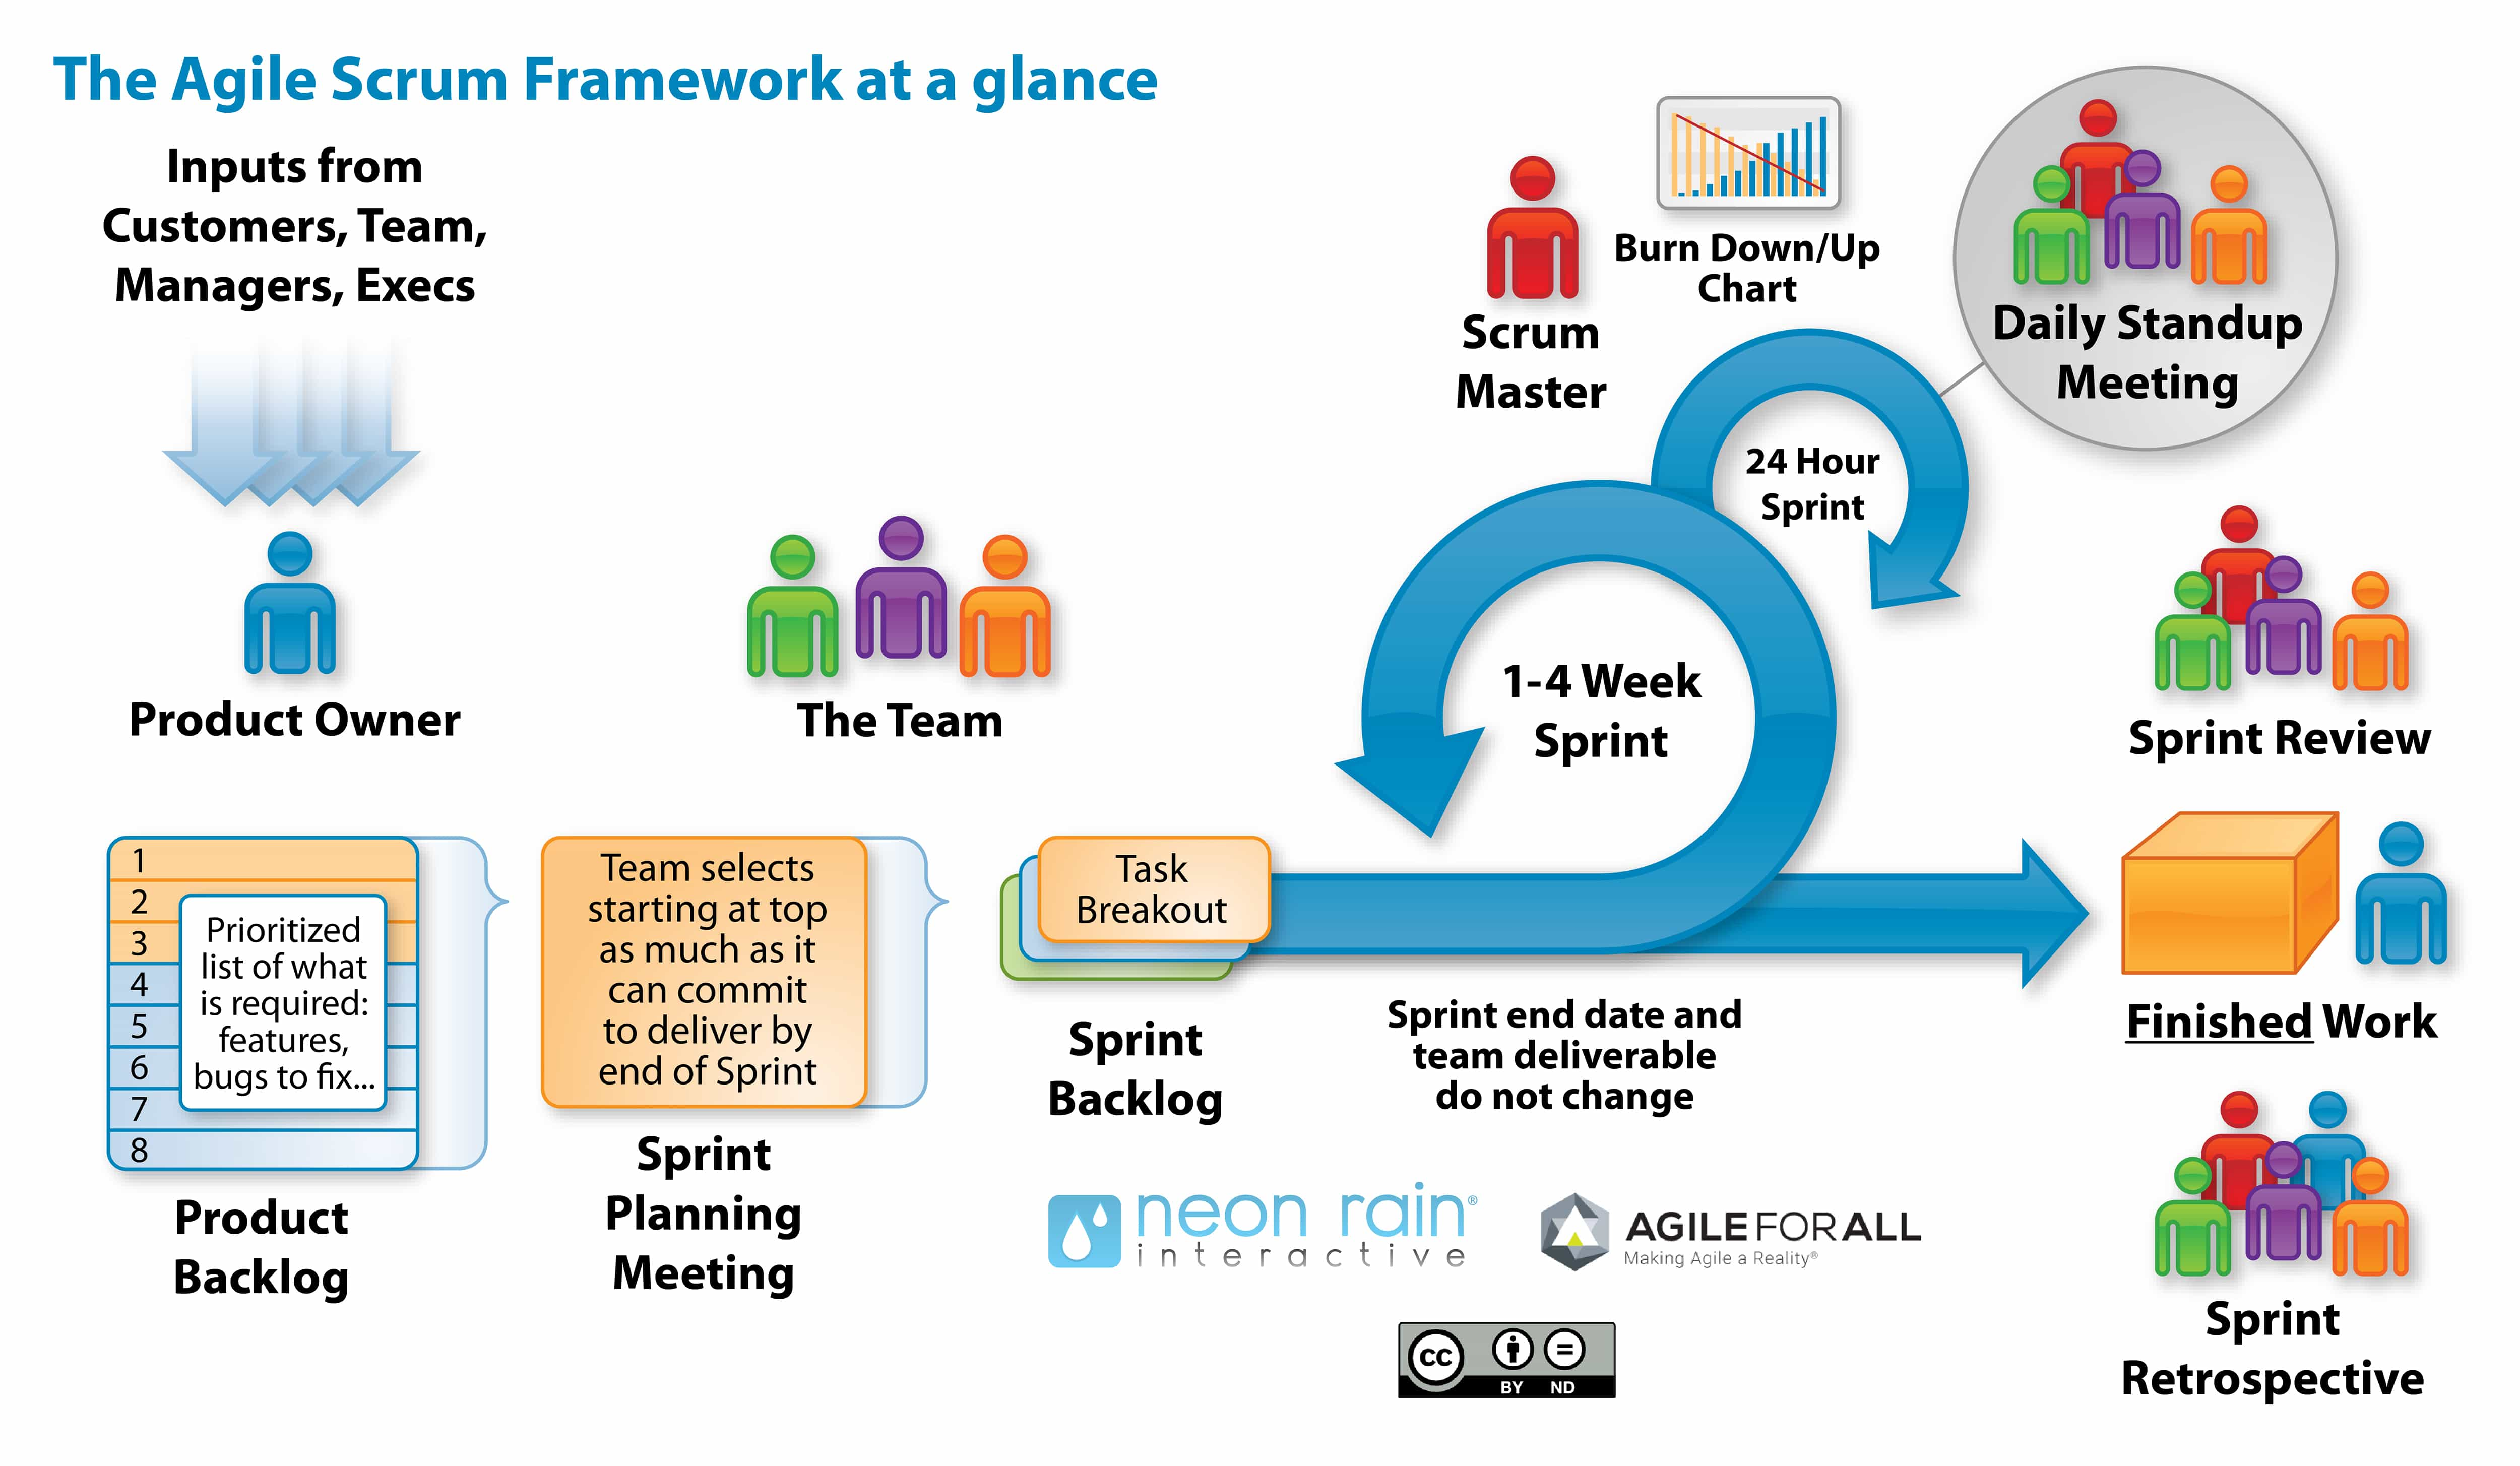
\includegraphics[width=1\textwidth]{./figures/chapter_02/07_scrum_framework.jpg}
  \setcaptioncitation{PENDIENTE}
  \caption{Scrum Framework}
  \label{fig:scrum_framework}
	\end{center}
\end{figure}

Los roles identificados en este metodología son:

\begin{description}[leftmargin=10em,style=nextline]
  \item[1. \textit{Stakeholder}] Corresponde a todas aquellas personas que se involucran en el proyecto, desde los usuarios finales hasta quienes financian el desarrollo del proyecto. Se identifica a todos aquellos que poseen algún interés una vez que el proyecto esté finalizado.
  \item[2. \textit{Product Owner}] Es el encargo de entender el contexto en el cual se desenvuelve el proyecto y en base a eso llevar a cabo el levantamiento de requerimientos del proyecto.
  \item[3. \textit{Scrum Master}] Es el responsable de verificar que la metodología Scrum sea aplicada de forma correcta, así como también el encargado de proporcionar a cada miembro del equipo los elementos que necesite para llevar a cabo su tarea. Este rol debe estar al servicio tanto del \textit{Product Owner} como para los miembros del equipo de desarrollo.
  \item[4. \textit{Development Team}] Son los responsables de la creación del proyecto en base a los requerimientos entregados por el \textit{Product Owner}.
\end{description}

Por su parte, la definición de los artefactos en esta metodología son:

\begin{description}[leftmargin=10em,style=nextline]
  \item[1. \textit{Product Backlog}] Es una lista ordenada de todas las necesidades del producto/proyecto y es la única fuente de requerimientos existente. El responsable de su escritura es el Product Owner, quien debe procurar por su contenido, disponibilidad y orden. Se debe indicar que nunca está completo y permanece en frecuente cambio frente a los diferentes requerimientos que el proyecto pueda ir necesitando. A modo general este artefacto posee las funcionalidades, requerimientos, mejoras y reparaciones para las próximas versiones del producto. Los elementos presentes poseen nombre o título, atributos que permiten describirlo, orden, estimación y valor para el proyecto \cite{scrum_guide}.
  \item[2. \textit{Sprint Backlog}] Es el conjunto de ítems seleccionados del Product Backlog que conforman el siguiente entregable del producto/proyecto que se está desarrollando. Se puede interpretar como la proyección de lo que será el software en su siguiente fase, donde todos los elementos presentes en este conjunto se considerarán terminados.
  \item[3. \textit{Increment}] Es la suma de todos los elementos desarrollados en un Sprint Backlog. Este debe considerarse terminado y listo para ser usado en la próxima versión del software.
\end{description}

Finalmente, se definen eventos dentro de Scrum con el objetivo de mantener una comunicación regular y eliminar la necesidad de encuentros. Cada evento posee una duración limitada y que puede varias según el proyecto así como también del equipo quien implemente la metodología, sin embargo, existen un periodo de tiempo recomendado en cada caso.

Los eventos presentes en Scrum son \cite{scrum_guide}:

\begin{description}[leftmargin=10em,style=nextline]
  \item[1. \textit{Sprint}] Se considera como el corazón de Scrum debido a que es el periodo de tiempo base en el cual se entrega un increment (incremento) del software. La duración recomendada para un sprint es un mes o semanas y es ideal que mantenga la misma duración durante todo el proyecto. Dentro de este periodo de tiempo ocurre el sprint planning, daily scrum, sprint review y, finalmente, sprint retrospective.
  \item[2. \textit{Sprint Planning}] Periodo de tiempo en el cual se planifica el trabajo y orden del mismo a realizarse en durante el sprint. El tiempo máximo para un sprint planning es de 8 horas cuando el tiempo del sprint es de un mes. El scrum master es el responsable de la gestión y la ejecución de esta fase. Por otro lado, se entiende que este periodo tiene por objetivo responder ¿qué elementos formarán parte del próximo increment ? y ,al mismo tiempo, ¿qué trabajo se realizará para cumplir el requerimiento descrito en el Product Backlog?

  \item[3. \textit{Dialy Scrum}] Consiste en una reunión de 15 minutos de duración donde el equipo de desarrollo sincroniza y crea el plan de desarrollo para las próximas 24 horas. Este trabajo se hace en base a la última reunión realizada. Adicionalmente, los miembros del equipo explican qué hicieron en el último daily scrum, que harán en el actual y de forma conjunta identifican e informan los problemas que han ocurrido y los que podrían ocurrir para el desarrollo del siguiente daily scrum.

  \item[4. \textit{Sprint Review}] Es una reunión informal con máxima duración de 4 horas donde los miembros del equipo de desarrollo identifican los logros obtenidos al final del sprint. Es una instancia en donde es posible modificar el Product Backlog. En esta reunión deben participan  stakeholders invitados por el Product Owner y todos los miembros de la metodología. Los principales objetivos de este intervalo de tiempo son:
    \begin{enumerate}
      \item Qué se hizo y qué no hizo.
      \item Se explican en detalle los problemas ocurridos y cómo fueron resueltos.
      \item Se discute de modo general qué elementos son importantes en base al avance logrado para el siguiente sprint planning.
      \item Se discute el estado del Product Backlog y se modifica en base al incremento logrado, a los cambios provenientes de los stakeholders así como también de los eventos externos del proyecto.
    \end{enumerate}

  \item[5. \textit{Sprint Retrospective}] Es un encuentro donde el equipo de desarrollo analiza su modo de trabajo y crea un plan de mejoras para ser atacadas en el próximo sprint. Se inspeccionan todos los ámbitos dentro de un equipo los miembros involucrados en el proyecto, relaciones entre ellos, procesos y herramientas utilizadas. Esta reunión se recomienda una duración máxima de 3 horas y se realiza al finalizar el sprint.
\end{description}

\subsubsection{Extreme Programming \label{sec:extreme_programming}}
Esta metodología basa su funcionamiento en 2 principios principales: simplicidad y eficiencia. Con el objetivo de lograr estos principios se definen los siguientes 4 valores o elementos, los cuales poseen sus propias características:

\begin{enumerate}
  \item \textbf{Comunicación (Communication)}\mbox{}\\ Enfocada en lograr la cooperación y buena relación entre los miembros del equipo, para lograr esto se propicia la participación constante del cliente, programación a pares y poseer dentro del equipo de desarrollo una estandarización de código.

  \item \textbf{Diseñar de modo simple (Simplicity)} \mbox{}\\ Orienta a que los elementos que se crean sean simples y basado en el pensamiento asociativo usando el mundo real como referencia, es decir, el uso de metáforas. Esto incluye las mejoras que se realizan a través de \textit{refactoring} \dictionary{refactoring}.

  \item \textbf{Retroalimentación constante (Feedback)} \mbox{}\\ Consiste en definir los modos para asegurarse que el software es aceptado tanto por el equipo de desarrollo como los clientes. Para ello necesita de testing continuo, integración continua (recomendado al menos una vez al día) y ,finalmente, basar las entregas en pequeñas funcionalidades.

  \item \textbf{Aceptación de nuevos cambios (Courage)} \mbox{}\\ Consta de todas las acciones usadas para la organización del proyecto y del equipo, para ello motiva realizar el levantamiento de requerimientos en base a relatos de usuario para el proyecto y a nivel de equipo estimula el concepto de propiedad de código colectiva.
\end{enumerate}

Los tiempos de desarrollo en XP se basan en iteraciones de 3 semanas en las cuales se recomienda seguir las siguientes 12 prácticas de software:

\begin{enumerate}
  \item Planificación del proceso : En esta instancia es donde se recomienda usar relatos de usuarios para la descripción de las funcionalidades del software.
  \item Entregables pequeños.
  \item Entregables pequeños.
  \item \textit{Test Driven Develpment} \dictionary{tdd}.
  \item \textit{Refactoring} \dictionary{refactoring}.
  \item Mantener el diseño simple.
  \item Programación a Parea \dictionary{pair_programming}.
  \item Propiedad colectiva del código.
  \item Uso de estándares de programación.
  \item Integración continua \dictionary{continuous_integration}.
  \item Mantener al cliente cercano.
  \item Mantener un buen clima laboral.
  \item Utilización de metáforas para el diseño : Consiste en crear un lenguaje común para el equipo de desarrollo y clientes con el objetivo de que todos puedan comprender los conceptos y definiciones usadas en el proyecto del mismo modo.
\end{enumerate}

La metodología es poco prescriptiva (en comparación a Scrum) pero existen prácticas sugeridas para organizar el flujo de trabajo. Por ejemplo, el sitio ExtremProgramming.Org sugiere el esquema presentado en la figura \ref{fig:extreme_programming_workflow}.

\begin{figure}[ht]
	\begin{center}
  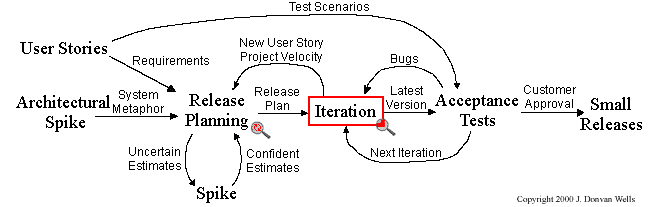
\includegraphics[width=1\textwidth]{./figures/chapter_02/08_extreme_programming_project.png}
  \setcaptioncitation{PENDIENTE}
  \caption{Flujo de Trabajo en \textit{Extreme Programming}}
  \label{fig:extreme_programming_workflow}
	\end{center}
\end{figure}

\subsection{Levantamiento de Requerimientos \label{sec:requirements}}

De acuerdo al Glosario Estándar de Ingeniería de Software de la IEEE \cite{ieee_glosary}, el concepto de requisito puede entenderse de acuerdo a alguna de las siguientes definiciones:

\begin{enumerate}
  \item Condición o capacidad necesaria por un usuario para solucionar un problema o alcanzar un objetivo.
  \item Condición o capacidad que debe ser encontrada o poseer un sistema o algún componente de éste que satisfaga un contrato, un estándar, especificación u otra formalidad impuesta por documentación.
\end{enumerate}

Al mismo tiempo, de acuerdo a la guía PMBOK \cite{pmbok_guide}, identifica 3 categorías:

\begin{enumerate}
  \item \textbf{Requerimientos del Negocio}\mbox{}\\ Describen las necesidades de alto nivel de la organización como un todo, tales como, oportunidades o problemas del negocio, y los motivos por los cuales un proyecto ha sido iniciado.
  \item \textbf{Requerimientos de los \textit{Stakeholders}}\mbox{}\\ Describen las necesidades de uno o varios \textit{stakeholders}.
  \item \textbf{Requerimientos de la Solución} \mbox{} \\ Describen las funcionalidades, funciones o características de un producto, servicio o resultado que resuelve los requerimientos del negocio y de los stakeholder. Dentro de los requerimientos de solución es posible encontrar dos tipos:
    \begin{enumerate}
      \item \textbf{Requerimientos funcionales:} Describen el comportamiento del producto o desarrollo. Por ejemplo: procesos, información, base de datos e interacciones del usuario y producto.
      \item \textbf{Requerimientos no funcionales:} Entrega los criterios medibles a través de los cuales un sistema puede comprobar su funcionamiento. Las principales áreas en las cuales se definen estos criterios son rendimiento, nivel de seguridad, escalabilidad, entre otros.
    \end{enumerate}
\end{enumerate}

Por lo descrito anteriormente, las metodologías permiten la captura de requisitos de diferentes maneras, las más usuales para los requerimientos del negocio y \textit{stakeholders} corresponden a \textit{focus groups} \dictionary{focus_group}, reuniones y encuestas. De modo transversal a las metodologías, este procedimiento de entendimiento donde se desarrolla el producto o \textit{software} finaliza con un objetivo principal y una serie de objetivos secundarios que deben cumplirse al término de éste. Esta dinámica en las metodologías mencionadas anteriormente se realiza en una etapa específica o designa un responsable para ello, por ejemplo, en Scrum el responsable de este procedimiento durante todo el proyecto es el \textit{Product Owner}. Adicional a esto, al momento de especificar los requerimientos de solución, debido a que los requisitos funcionales describen comportamiento, el cual dentro de lo posible debe ser interpretado del mismo por todo los miembros del equipo, presentan la necesidad de realizarse bajo una estructura o esquema de descripción específico. Esta situación no sucede con los requerimientos no funcionales, debido a que ellos presentan métricas  y sus criterios para ser evaluadas , por ejemplo, el tiempo de carga al sitio inicial del \textit{software} no debe ser mayor a 1 segundo.

Dentro de las técnicas de descripción o \textbf{levantamiento de requisitos funcionales}, se encuentran Casos de Usos \textit{(Use Cases)} y Relatos de Usuarios \textit{(User Stories)}.

\subsubsection{Casos de Uso \label{sec:use_cases}}

De Acuerdo a Cockburn \cite{uses_cases_writing}, un caso de uso se define como la descripción del comportamiento del sistema bajo varias condiciones que responden a la necesidad de uno o varios \textit{stakeholders}. Adicionalmente, se espera que un caso de uso sea fácil de leer, para una completa identificación de las necesidades se propone las siguientes partes para una descripción completa:

\begin{enumerate}
  \item \textbf{Nombre \textit{(Name)}}\mbox{}\\ Correspondiente al nombre de la acción que se desea realizar.
  \item \textbf{Objetivo en Contexto \textit{(Goal in Context)}}\mbox{}\\ Menciona las motivaciones del actor principal para la realización de sus acciones, así como también la descripción del entorno en el cual las realiza.
  \item \textbf{Alcance del diseño \textit{(Design Scope)}} \mbox{} \\ Corresponde a la definición de que se desarrolla y no desarrolla dentro del proyecto. Con el objetivo de describir el alcance dentro de un contexto Cockburn define los siguientes niveles o tipos de alcance:
    \begin{enumerate}
      \item \textbf{Corporativo \textit{(Corporative)}:} Indica que la discusión para definir el alcance envuelve al comportamiento de toda la organización. Por ejemplo, cuando se debe entregar un desarrollo a un agente externo al contexto del proyecto.
      \item \textbf{Sistema \textit{(System)}:} Corresponde sólo a una parte del producto o software que se está construyendo.
      \item \textbf{Sub sistema \textit{(Sub system)}:} Si bien Cockburn indica que a un alcance de sistema debería bastar para la descripción de un software. En caso de que se requiera dividir una pieza de software en varias partes recomienda ocupar la categoría de sub sistema para ella.
    \end{enumerate}
  \item \textbf{Niveles de los objetivos} \mbox{} \\ Corresponde al nivel de especificidad que se declara en un objetivo.A continuación se enuncian los niveles existentes:
    \begin{enumerate}
      \item \textbf{\textit{Very High Summary}} Indica la razón principal de las acciones del usuario principal.
      \item \textbf{\textit{Summary}} Describe un global más global que puede abarcar diferentes visiones provenientes de diferentes actores principales.
      \item \textbf{\textit{User-goal level}} Corresponde a una descripción amplia de lo que se desea lograr. Esta descripción o deseo se hace a nivel del actor principal del caso de uso, por lo tanto, indica un nivel de agrupación de objetivos secundarios identificados como \textit{subfunction}.
      \item \textbf{\textit{Subfunction}} Corresponde al conjunto de objetivos obligatorios que deben cumplirse poder alcanzar otros objetivos de nivel superior. A este nivel un objetivo secundario ya es posible identificarlo como una acción clara del usuario.
      \item \textbf{\textit{Too Low}} Corresponde a un nivel de objetivos más abajo que subfunction y agrupan todas las tareas más básicas que deben realizarse lograr el objetivo planteado.

      El esquema \ref{fig:use_cases_levels} permite visualizar de forma gráfica un ejemplo de los niveles mencionados.

      \begin{figure}[ht]
      	\begin{center}
        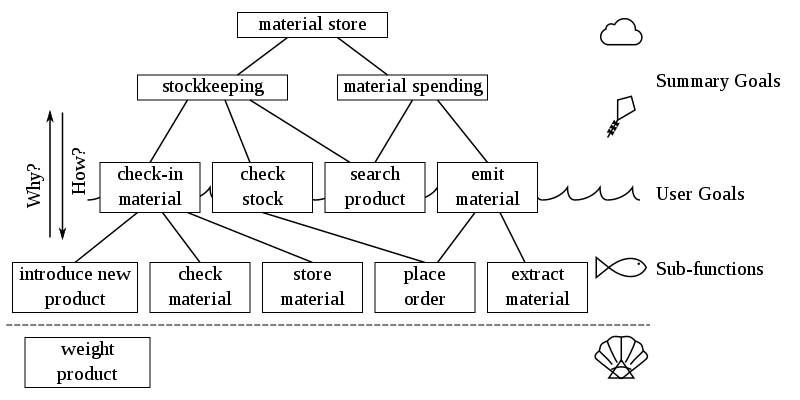
\includegraphics[width=1\textwidth]{./figures/chapter_02/09_cockburnstyle_use_cases.png}
        \setcaptioncitation{PENDIENTE}
        \caption{Niveles de los Objetivos}
        \label{fig:use_cases_levels}
      	\end{center}
      \end{figure}

      \item \textbf{Actor Principal \textit{(Principal Actor)}:} Indica al usuario que realiza o ejecuta el conjunto de acciones indicadas por el caso de usuario. Si bien Cockburn menciona en esta versión de caso de uso sólo un actor dentro del caso de uso, es posible incluir otros como actores secundarios.
      \item \textbf{\textit{Stakeholders} e intereses \textit{(Stakeholders and Interests)}:} Se atribuye al conjunto de stakeholder y los objetivos que cada uno busca.
      \item \textbf{Precondiciones \textit{(Preconditions)}:} Corresponden al conjunto de elementos que se deben cumplir antes de iniciar el flujo de etapas del caso de uso.
      \item \textbf{Estado de éxito \textit{(Success End Condition)}:} Muestra el estado en el cual el sistema se encuentra de la una ejecución exitosa del caso de uso.
      \item \textbf{Estado de error \textit{(Failed End Protection)}:} Describe el estado del sistema en caso de no alcanzar el objetivo.
      \item \textbf{\textit{Trigger}:} Corresponde a la acción que desencadena  el caso de uso.
      \item \textbf{Descripción \textit{(Description)}:} Conjunto de pasos a seguir para alcanzar el objetivo del caso de uso.
      \item \textbf{Extensiones \textit{(Extensions)}:} Corresponde a un flujo adicional que puede ser el caso de uso al momento de darse un condición especial sobre el sistema o los actores involucrados.
      \item \textbf{Variaciones \textit{(Variants)}:} Indica la ejecución de una misma acción de un modo distinto dentro del sistema , por ejemplo, al momento de pagar puede realizarse a través de dinero en efectivo, transferencia bancaria, entre otros.
    \end{enumerate}
\end{enumerate}

La lista anteriormente descrita puede verse resumida en el recuadro \ref{fig:uses_cases_summary} conocido por Cockburn \cite{uses_cases_writing} como la versión completamente vestida (fully dressed).

\begin{figure}[ht]
  \begin{center}
  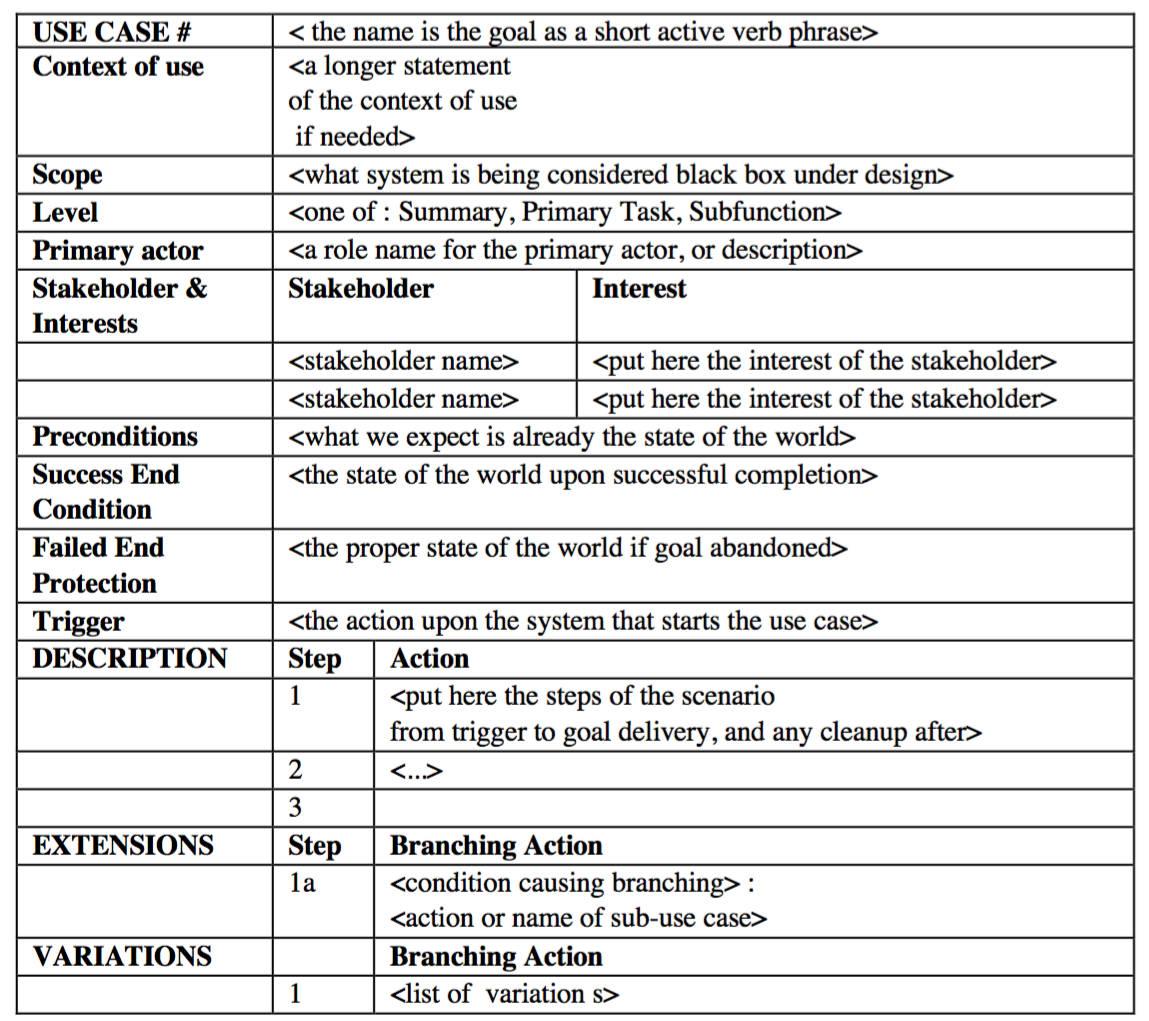
\includegraphics[width=0.8\textwidth]{./figures/chapter_02/10_use_case_template_one_column_version.png}
  \setcaptioncitation{PENDIENTE}
  \caption{Versión de Caso de Uso de una columna}
  \label{fig:uses_cases_summary}
  \end{center}
\end{figure}

Adicionalmente a lo descrito anteriormente, con el objetivo de tener una mejor visualización de la interacción entre casos de usos y actores principales como secundarios el \textit{Unified Modeling Language (U.M.L.)} \cite{uml} entrega los estándares y elementos para realizar la diagramación de un caso de uso. Este tipo de diagrama se denomina use case view o vista de un caso de uso. Los elementos presentes en esta visualización se aprecian en la representación gráfica de un caso de uso (figura \ref{fig:use_case_view}).

\begin{figure}[ht]
  \begin{center}
  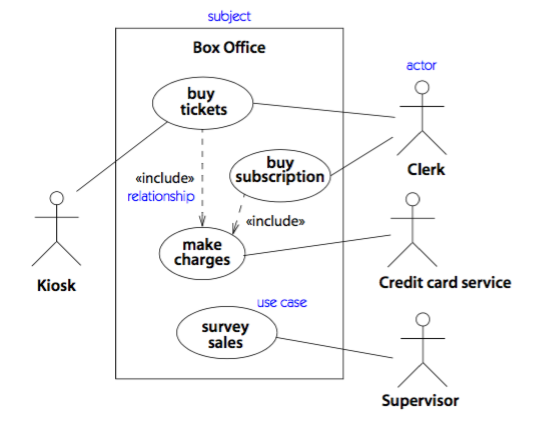
\includegraphics[width=0.8\textwidth]{./figures/chapter_02/11_use_case_view.png}
  \setcaptioncitation{PENDIENTE}
  \caption{Representación Gráfica de un Caso de Uso}
  \label{fig:use_case_view}
  \end{center}
\end{figure}

De este modo, para lograr la descripción de un caso de uso, se necesita tanto su diagrama descrito en UML como su detalle, el cual puede estar basado en la estructura propuesta por Cockburn o una estructura similar, pero más simple.

\subsubsection{Relatos de Usuarios \label{sec:user_stories}}

Según Mike Cohn \cite{user_stories_applied}, un relato de usuario describe una funcionalidad que es valorada por un usuario o otro sistema que se alimenta de ella.  Las partes de un relato consisten en la identificador,descripción de la funcionalidad, los criterios de aceptación, prioridad para el negocio y el puntaje de dificultad identificado por el equipo desarrollador. Adicional a lo anterior, cada relato de usuario debe cumplir las siguientes propiedades:

\begin{enumerate}
  \item \textbf{Independiente:} Un relato de usuario es independiente de los demás.
  \item \textbf{Negociable:} No son contratos , por lo que puede ser discutida y descrita por todos los \textit{stakeholders} y los miembros del equipo desarrollador.
  \item \textbf{Valorada por los compradores y por los usuarios:} Indica que las características del software descrito debe agregar valor tanto para las personas que lo ocupan como aquellas que “pagan” por él.
  \item \textbf{Estimable:} Es importante poder asignarle un tamaño al relato de usuario para identificar la cantidad de tiempo que tomará. Se indica que un relato que no es posible estimarlo es demasiado grande y es recomendable subdividirlo en varios.
  \item \textbf{Pequeña:} Indica que la descripción de un relato de un usuario no puede ser tan general porque en caso de ser así no podrá ser estimada de forma adecuada. En caso de suceder esto, se recomienda agruparlas bajo un epic \dictionary{epic} y que la funcionalidad  sea dividida en relatos de usuarios más pequeños y con mayor cantidad de detalle.
  \item \textbf{Comprobable:} Indica que debe existir una forma concreta y no general de que el relato de usuario se desarrolló de forma exitosa.
\end{enumerate}

Con el objetivo de que el relato de usuario pueda cumplir con las propiedades descritas anteriormente, Cohen recomienda utilizar el formato de tarjeta para su descripción. La ilustración \ref{fig:user_story_structure} ilustra esta propuesta.

\begin{figure}[ht]
  \begin{center}
  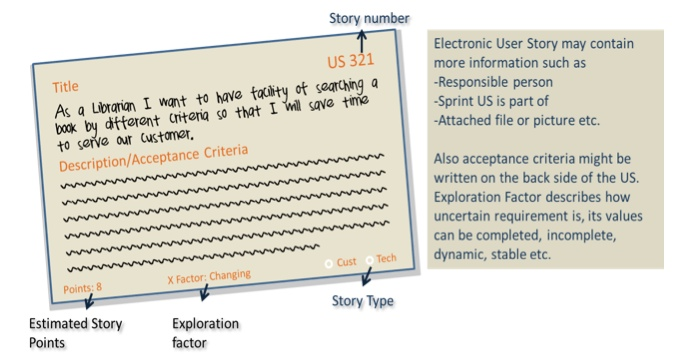
\includegraphics[width=1\textwidth]{./figures/chapter_02/12_yodiz_user_story_card.jpg}
  \setcaptioncitation{PENDIENTE}
  \caption{Estructura de un relato de Usuario}
  \label{fig:user_story_structure}
  \end{center}
\end{figure}

\begin{enumerate}
  \item \textbf{Identificador:} Compuesto por un número o nomenclatura con el formato US-XX, donde XX corresponde al número del relato.
  \item \textbf{Título:} Describe la funcionalidad que se debe desarrollador. El título debe posee el siguiente formato
    \begin{center}
      	As a \textbf{<type of user>}, I want \textbf{<some goal>} so that \textbf{<some reason>}.
    \end{center}

  Cohen \cite{user_stories_applied} indica que la parte <some reason> en muchos casos es opcional.
  \item \textbf{Puntaje:} Correspondiente al grado de dificultad del relato. Se espera que un relato de 2X tome el doble de tiempo que uno de X puntos.
  \item \textbf{Prioridad:} Indica el orden en el cual deben ser desarrolladas los relatos de usuarios.
  \item \textbf{Criterios de Aceptación:} Corresponde a las condiciones que debe cumplir el relato de usuario. No se especifica un formato para escribir un criterio de aceptación, pero se recomienda que indique de forma precisa lo que se espera del software, por ejemplo, el sistema debe solicitar el nombre, apellido y correo electrónico para poder identificar a un usuario.
\end{enumerate}

Otro punto importante que destaca Cohn es el uso de \textit{epics} \dictionary{epic}, él indica que no existe un criterio universal para clasificar una historia de usuario como grande, pero sí deben buscar cumplir del mejor modo las propiedades anteriormente descritas. Frente a la necesidad de agrupar, dos o más relatos de usuarios bajo un mismo concepto es cuando se hace el uso de un epic, el cual posee simplemente un nombre relativo a la funcionalidad que describe,una descripción para dar más contexto a quien lee la documentación del proyecto y un código identificador para realizar mejor el agrupamiento de los relatos de usuarios descritos anteriormente \cite{user_stories_applied}.

\subsection{Metodología y técnicas usadas en este trabajo \label{sec:work_decisions}}

Dentro de las metodologías y técnicas para levantamiento de requisitos descritas anteriormente para este proyecto se escogió la metodología XP y levantamiento de requisitos funcionales vía relatos de usuario. Se consideró que para la implementación de Scrum se hacía necesario incorporar un Product Owner, y un Scrum Master además de los miembros de equipo de desarrollo. XP es menos prescriptivo y permite organizar el  trabajo en función de la experiencia del equipo de desarrollo, siempre y cuando, se respeten los principios que ésta estipula.  Otro factor  que se tuvo en cuenta es que dada la considerable complejidad del problema, lo que buscábamos es más bien producir un primer prototipo o lo que se conoce como un \textit{Minimal Viable Product}, en adelante MVP \dictionary{mvp}. XP gracias a su principio  de simplicidad (Simplicity) permite abordar de mejor manera este escenario.

Por otro parte, a nivel de levantamiento de requisitos si bien tanto Casos de Usos como Relatos pueden ser aplicados con metodologías ágiles, se escogió relatos de usuario debido a su naturaleza menos estructurada que privilegia la comprensión de los requisitos en base a conversaciones con los  stakeholder Adicionalmente a lo anterior, las propiedades de los relatos de usuarios (independiente, negociable, valorado por los usuarios o compradores, estimable, pequeña y comprobable) permite un mejor registro de los esfuerzos invertidos en el desarrollo del prototipo.

Finalmente, el hecho de que el formato de los relatos de usuarios marque explícitamente el objetivo que se buscar resolver permite una mejor visualización general de las soluciones implementadas y al mismo tiempo permite llevar un control efectivo del avance del proyecto de modo más sencillo en base a cada uno de los artefactos requeridos por éste.

\section{Descubrimiento de Conocimiento (Knowledge Discovery) \label{sec:knowledge_discovery}}
Fayyad \cite{knowledge_discovery} en 1996 define término Knowledge Discovery como el conjunto de conocimientos relativos al proceso de extracción, almacenamiento y accesibilidad de datos; el uso de algoritmos ,en forma eficiente, para el análisis de los mismos; y, finalmente, la interpretación y visualización de resultados en base a estos, este resultado es conocido como \textit{knowledge}(conocimiento).

\subsection{Categorías, metodologías y modelos \label{sec:problem_categories}}
Desde la creación de este término hasta hoy en día han surgido varias metodologías para llevar a cabo el proceso anteriormente descrito, el cual se denomina \textit{Knowledge Discovery Process (KDP)}. Se logran logran identificar un total de 4 \cite{knowledge_discovery}:

\begin{enumerate}
  \item \textbf{\textit{Traditional KDP Approach}}\mbox{}\\ Agrupa aquellas metodologías que ocupan un proceso similar al propuesto por Fayyad et al., los cuales poseen las etapas de entendimiento del negocio, entendimiento de los datos, procesamientos de los datos, modelamiento o minería de datos, evaluación de modelos y ,finalmente, paso a producción o visualización. La característica principal de estas metodologías es que consisten en etapas secuenciales y sin mucha flexibilidad para la aceptación de cambios. La figura \ref{fig:traditional_kdd_structure} permite la visualización de la secuencia de etapas.

  \begin{figure}[ht]
    \begin{center}
    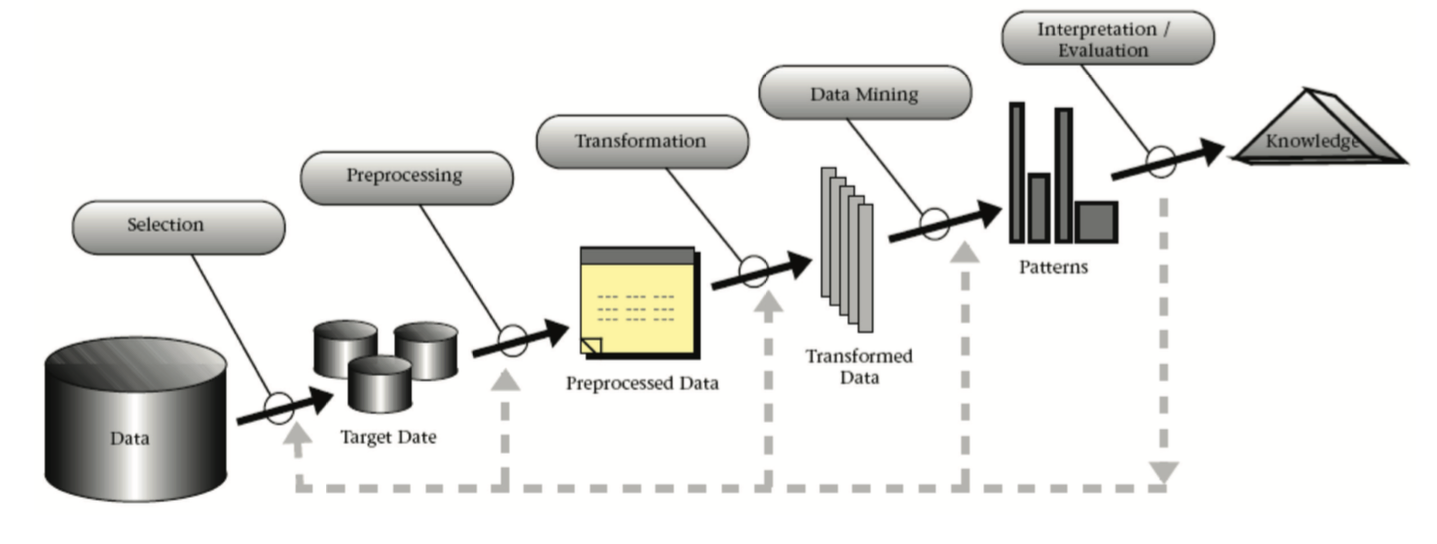
\includegraphics[width=1\textwidth]{./figures/chapter_02/13_kdd_process_model.png}
    \setcaptioncitation{PENDIENTE}
    \caption{Etapas del proceso tradicional de KDD}
    \label{fig:traditional_kdd_structure}
    \end{center}
  \end{figure}

  \item \textbf{\textit{Ontology-based KDP Approach}}\mbox{}\\ Se basa en la mezcla de ingeniería ontológica \dictionary{ontoligical} y un enfoque tradicional para KDP.
  \item \textbf{\textit{Web-based KDP Approach}} \mbox{} \\ Incorpora las mismas etapas que la primera categoría, pero reconoce de forma especial a la información proveniente de \textit{web logs} y ,por lo mismo, define etapas precisas para el tratamiento de la misma.
  \item \textbf{\textit{Agile-based KDP Approach}} \mbox{} \\  Esta categoría agrupa aquellos modelos que incorporan metodologías ágiles a un enfoque tradicional para KDP.
\end{enumerate}

\subsubsection{Modelos \label{sec:knowledge_discovery_models}}

Los mismos autores mencionados anteriormente, Mouhib y Asim, reconocen al mismo al mismo tiempos 9 modelos considerados líderes a lo largo de la historia de KDP, estos modelos son:

\begin{tabularx}{\linewidth}{@{}Y  Y  Y  Y@{}}
  \caption{Modelos a lo largo de la historia de \textit{KDP}} \label{tab:kdp_models}\\
  \toprule
  Nombre	&	Autor	&	Año de Creación
  \endhead
  \midrule
  Knowledge Discovery in Databases (KDD) Process & Fayyad et al. & 1996 \\
  \midrule
  Information Flow in a Data Mining Life Cycle & Ganesh et al. & 1996 \\
  \midrule
  SEMMA & SAS Institute & 1997 \\
  \midrule
  Refined KDD paradigm & Collier et al. & 1998 \\
  \midrule
  Knowledge Discovery Life Cycle (KDLC) Model & Lee and Kerschberg & 1998 \\
  \midrule
  CRoss-Industry-Standard Process for Data Mining (CRISP-DM) & CRISP-DM & 2000 \\
  \midrule
  Generic Data Mining Life Cycle by (DMLC) & Hofmann & 2003 \\
  \midrule
  Ontology Driven Knowledge Discovery Process (ODKD) & Gottgtroy & 2007 \\
  \midrule
  Adaptive Software Development-Data Mining (ASD-DM) Process Model & Alnoukari et al. & 2008 \\
\end{tabularx}

Dentro de todos los modelos mencionados anteriormente se consideran relevantes para el presente trabajo CRISP-DM y ASD-DM, los cuales se describen las siguientes secciones.

\subsubsection{CRISP-DM \label{crip_dm}}
Este fue uno de los primeros modelos que intentó abarcar la problema impuesta por el área de \textit{Knowledge Discovery}. Para lograr lo anterior este modelo define 4 niveles de abstracción, en los cuales se realizan actividades, las cuales a su vez pertenecen a una de las 6 fases específicas por las cuales pasa todo proceso. La ilustración \ref{fig:hierarchical_activity_levels} muestra los 4 niveles creados en este modelo.

\begin{figure}[ht]
  \begin{center}
  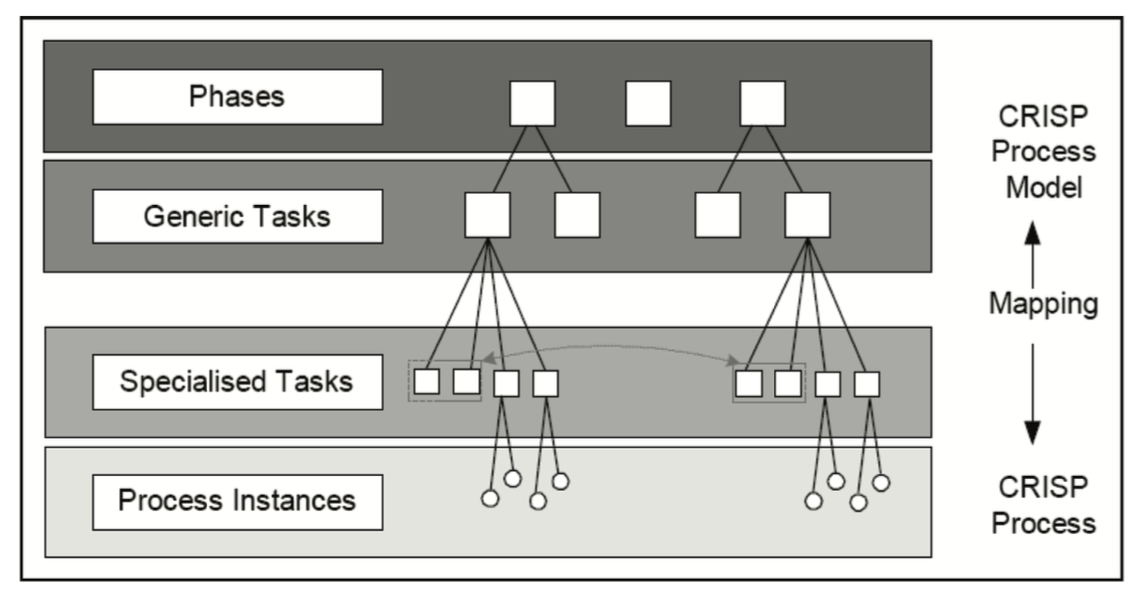
\includegraphics[width=1\textwidth]{./figures/chapter_02/14_crips_dm_hierarchical_process_model.png}
  \setcaptioncitation{PENDIENTE}
  \caption{Niveles de Categorización de Actividades en CRISP-DM}
  \label{fig:hierarchical_activity_levels}
  \end{center}
\end{figure}

Dentro de cada nivel se deben definir actividades, las cuales a su vez se encuentran categorizadas y divididas al mismo tiempo en sub tareas para poder llevarse a cabo. La intención de estos niveles jerárquicos es poder tener una clara agrupación de qué tareas específicas se realizan en cada proceso utilizada para la generación de conocimiento. Por otro lado, no existe un listado de actividades o tareas específicas que se deban realizar en cada uno de los niveles, sólo se espera que las tareas en las fases que se ilustran en el diagrama \ref{fig:crisp_dm_phases} contengan sus tareas o actividades categorizadas en los niveles previamente mencionados.

\begin{figure}[ht]
  \begin{center}
  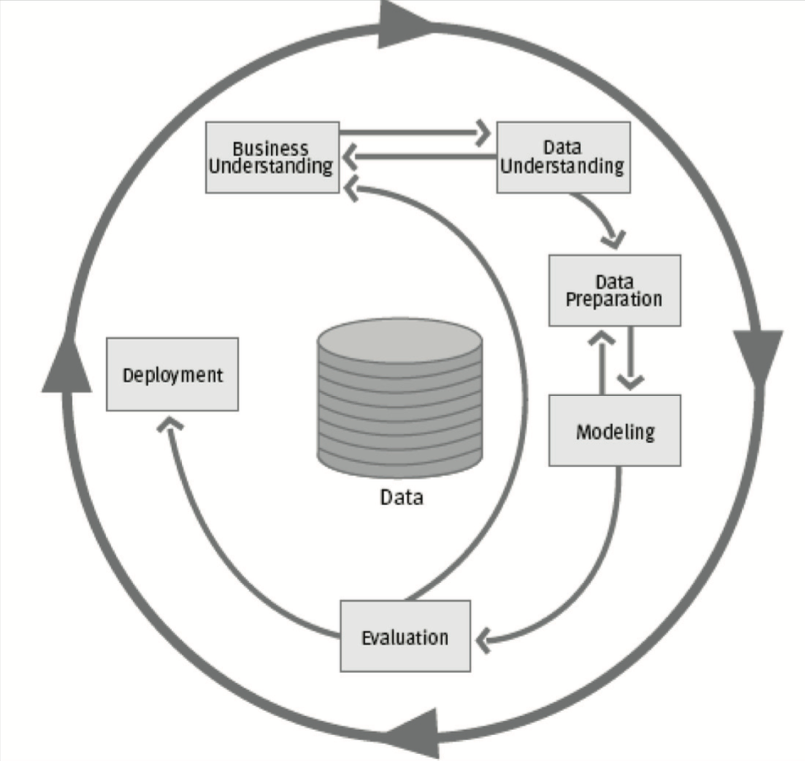
\includegraphics[width=0.6\textwidth]{./figures/chapter_02/15_crips_dm_phases.png}
  \setcaptioncitation{PENDIENTE}
  \caption{Fases en CRISP-DM}
  \label{fig:crisp_dm_phases}
  \end{center}
\end{figure}

Por la definición de estas fases se considera que este modelo posee un enfoque tradicional para KDP. Es posible establecer las siguientes definiciones para cada una de las fases ilustradas anteriormente \cite{knowledge_discovery}:

\begin{enumerate}
  \item \textbf{\textit{Business Understanding}:} Consiste en el entendimiento de los requerimientos generales del contexto en el cual se desenvuelve el proyecto así. En base a lo anterior, se crea una lista de objetivos que puedan ser respondidos por minería de datos y ,finalmente, elemento se crea una planificación general del proyecto.
  \item \textbf{\textit{Data Understanding}:} Esta etapa concierne específicamente a la recolección de los datos iniciales, descripción de ellos a través de metadata, exploración y verificación de la calidad de los mismos.
  \item \textbf{\textit{Data Preparation}:} Corresponden a todas las actividades necesarias para la creación del conjunto de datos final que será utilizada en la siguiente fase de modelamiento y análisis. Se encuentra dividido en : selección, limpieza, construcción, integración y formateo de datos.
  \item \textbf{\textit{Modeling}:} Orientado a la selección y aplicación apropiada de técnicas de modelamiento y minería de datos. Se encuentra seccionado en las fases de selección de técnicas de modelamiento, generación de pruebas, creación de modelos y ,finalmente, evaluación de los modelos generados.
  \item \textbf{\textit{Evaluation}:} Relacionado a la evaluar si el modelo escogido cumple con los objetivos impuestos en la primera fase.
  \item \textbf{\textit{Deployment}:} Etapa relacionada a la instalación a todo lo necesario para que el conocimiento generado puede ser ocupado por los usuarios finales. Esta etapa se caracteriza por presentar las siguientes fases: plan de instalación, plan de monitoreo y mantenimiento, generación de un reporte final donde se explica lo realizado y revisión de los pasos a seguir, en caso de ser requerido, de lo contrario, la finalización del proyecto.
\end{enumerate}

\subsubsection{Adaptative Software Development - Data Minning (ASD-DM) \label{asd_dm}}

Este modelo se caracteriza por la incorporación de elementos presentes en metodologías ágiles para los proyectos de minería de datos. La idea basal sobre esta filosofía es que un enfoque adaptativo (flexible y/o incremental) posee un mejor rendimiento al momento de trabajar con requerimientos desconocidos o cambiantes, efecto que no es posible resolver de forma eficiente en los enfoques tradicionales de KDP.

Para lograr su objetivo, este modelo \cite{knowledge_discovery} define 6 etapas organizadas en 3 fases que se muestran en el diagrama \ref{fig:adm_dm_phases}.

\begin{figure}[ht]
  \begin{center}
  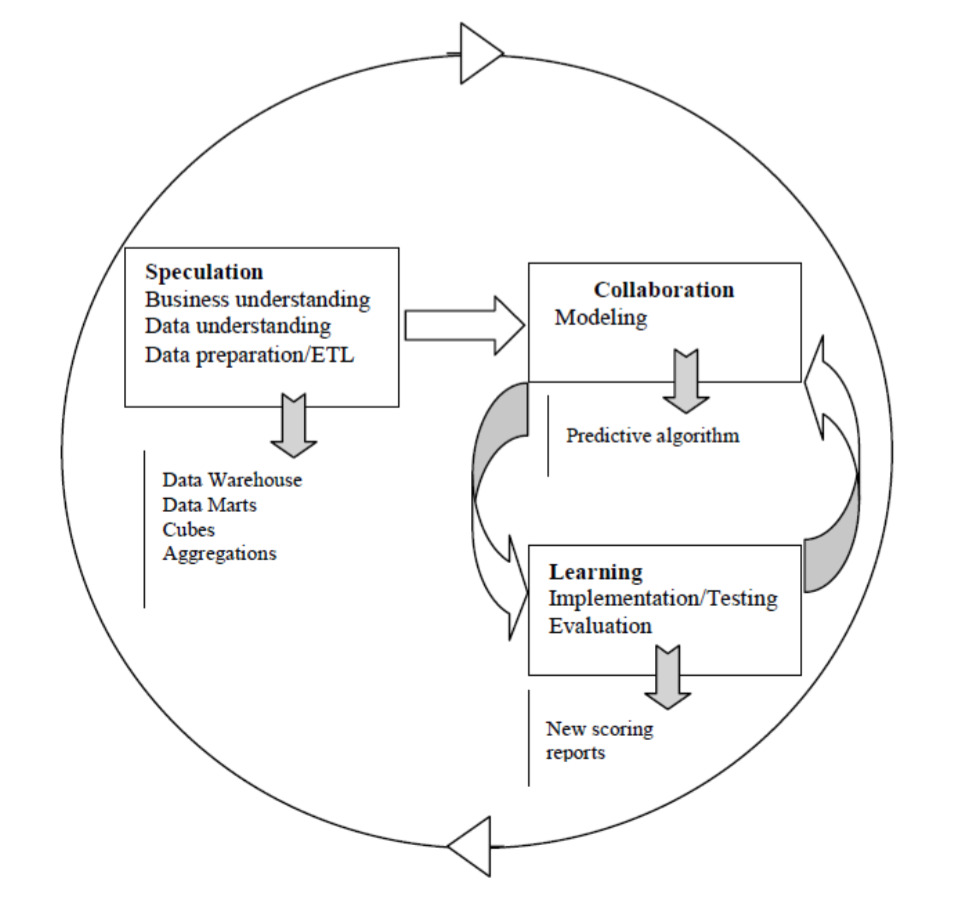
\includegraphics[width=0.6\textwidth]{./figures/chapter_02/16_asm_dm_process_model_phases.png}
  \setcaptioncitation{PENDIENTE}
  \caption{Fases en ASM-DM}
  \label{fig:adm_dm_phases}
  \end{center}
\end{figure}

Las etapas presentadas anteriormente pueden definirse del siguiente modo:

\begin{enumerate}
  \item \textbf{Etapa de Especulación \textit{(Speculation)}:} Incluye todas actividades que se necesiten realizar para el entendimiento del negocio y la preparación de los datos. Esta etapa termina cuando se han creado las fuentes de información en forma de \textit{data warehouse}, \textit{data marts}, cubos o agrupaciones de los datos.
  \item \textbf{Etapa de Colaboración \textit{(Collaboration)}:} Propicia toda actividad en donde se involucre a los stakeholders del proyecto para así poder escoger el mejor modelo para realizar la predicción posible.
  \item \textbf{Etapa de Aprendizaje \textit{(Learning)}:} Orientada a definir las tareas de pruebas y evaluación de los resultados obtenidos por el o los modelos escogidos en la fase anterior. En caso de ser los resultados aceptados por los \textit{stakeholders}, se procede a la entrega de un reporte final con los resultados explicados, de contrario, se vuelve a la fase anterior.
\end{enumerate}

\subsection{Metodologías y modelos usadas en este trabajo \label{sec:problem_categories}}

Si bien la metodología CRISP-DM presenta muchas de las cualidades que se necesitan para el desarrollo de este proyecto, no era la metodología más adecuada debido  a que incluye una claro paso a producción una vez que la etapa de evaluación haya llegado a su fin. El objetivo de este proyecto es poder presentar una primera solución al cálculo de la demanda de cursos del nuevo currículum de estudios, el cual aún no posee datos suficientes para poder realizar una generalización de datos para los próximos años. Frente a esta situación, se hace necesario que el proceso de aprendizaje se haga de un modo más continuo y que la nueva información que se vaya consiguiendo en el tiempo permita mejorar los niveles de predicción obtenidos. Teniendo en cuenta estos objetivos, se consideró que la metodología \textit{Adaptive Software Development-Data Mining} era la apropiada  gracias a la interacción continúa entre sus fases collaboration y learning, logrando así una incorporación de nuevos datos a medida que pase el tiempo e ir mejorando así los modelos predictivos creados.
